\documentclass[../main.tex]{subfiles}

\begin{document}

\section{Results}
We chose accuracy as our primary performance metric to evaluate our emotion 
classification model. This is because accuracy provides a straightforward 
measure of the proportion of correctly classified samples. Moreover, with a 
balanced dataset, accuracy alone is able to reflect the model's 
classification capability without requiring additional metrics like precision 
or recall.

\subsection{Baseline Performance}

A ResNet-based CNN from Torchvision was chosen as the baseline model, since it performs well in image-based tasks like spectrogram 
classification. It focuses solely on spatial feature 
extraction, and thus it is an appropriate point of comparison for our CRNN, 
which incorporates temporal modeling.

As shown in \autoref{fig:baseline_mixed}, the baseline model ended up performing much 
better than our CRNN model. It had a validation accuracy of 0.7830 and a 
test accuracy of 0.7899, which is an 18\% increase in accuracy when compared to 
our CRNN model.

\begin{figure}[h]
    \centering
    \begin{minipage}{.5\textwidth}
      \centering
      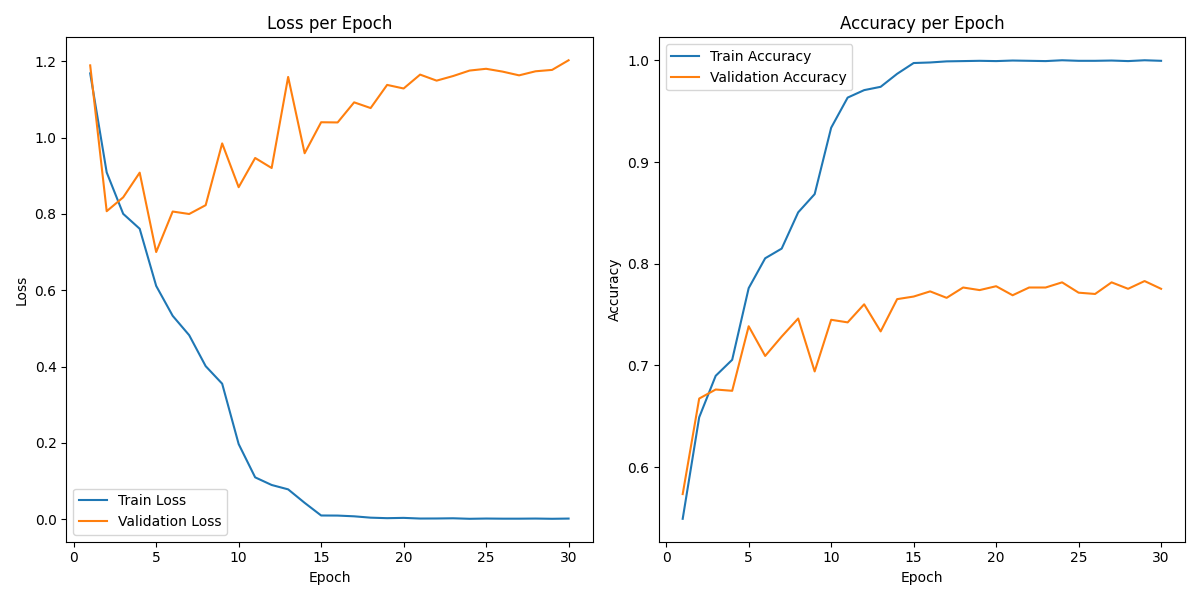
\includegraphics[width=1.0\linewidth]{../resources/baseline_mixed.png}
      \caption{Traing and validation accuracy of ResNet-based CNN baseline model
      along with loss.}
      \label{fig:baseline_mixed}
    \end{minipage}%
    \hfill
    \begin{minipage}{.4\textwidth}
      \centering
      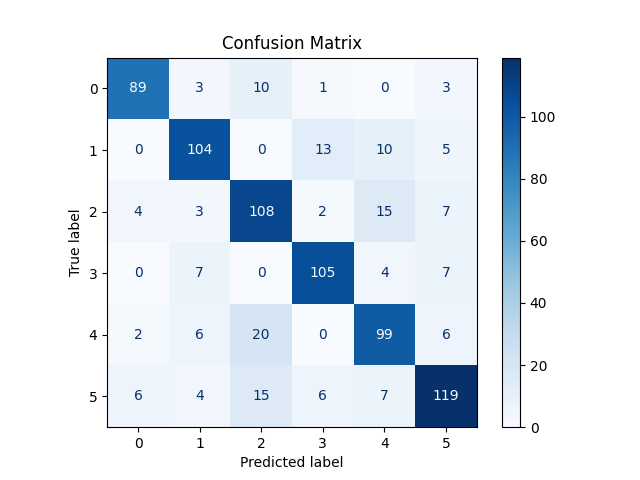
\includegraphics[width=1.0\linewidth]{../resources/baseline_confusion.png}
      \caption{Confusion matrix of ResNet-based CNN baseline mode. The six categories (0-5) 
      represent the emotions neutral (0), happy (1), sad (2), anger (3), fear (4), 
      and disgust (5).} 
      \label{fig:baseline_confusion}
    \end{minipage}
\end{figure}


\subsection{CRNN Performance}
% Our original plan with the CRNN model was to use it on waveforms, but this 
% strained memory and made preprocessing too intensive on the fly. To address 
% this, we decided to save Mel-spectrograms and test them with our CRNN model, 
% but it didn't perform as well as we expected it to. 

After training our model on three datasets (TESS, CREMA-D, and RAVDESS), our 
CRNN model achieved a validation accuracy of 0.64\% and a test accuracy of 61\%
as shown in \autoref{fig:crnn_graph_mixed}.

\begin{figure}[h]
    \centering
    \begin{minipage}{.5\textwidth}
      \centering
      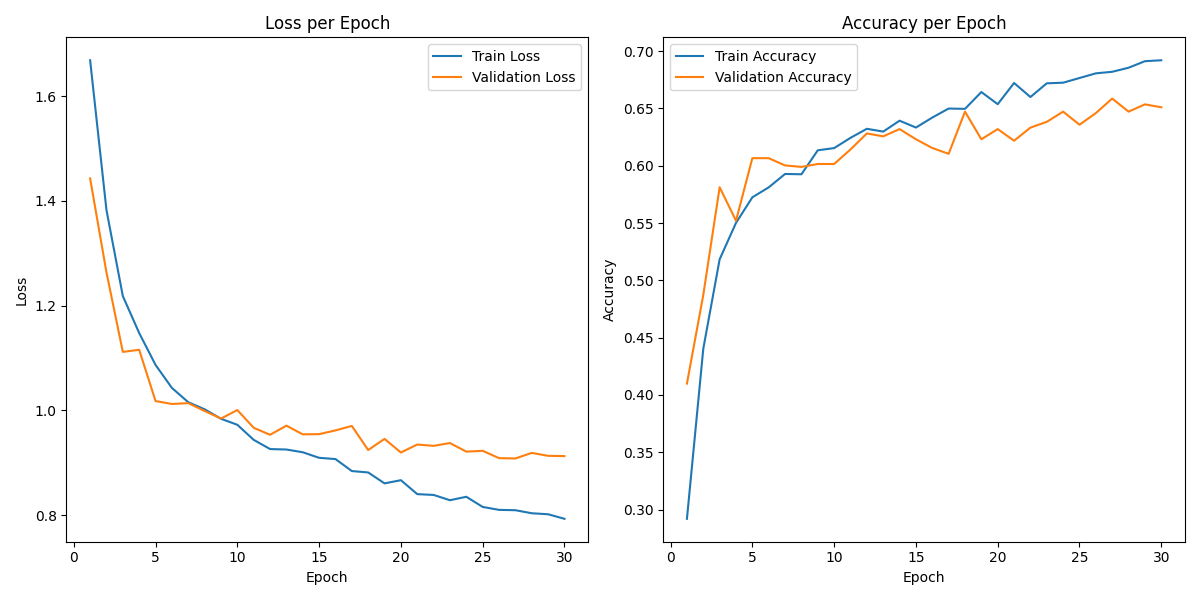
\includegraphics[width=1.0\linewidth]{../resources/crnn_graph_mixed.png}
      \caption{Traing and validation accuracy of CRNN model along with loss.}
      \label{fig:crnn_graph_mixed}
    \end{minipage}%
    \hfill
    \begin{minipage}{.4\textwidth}
      \centering
      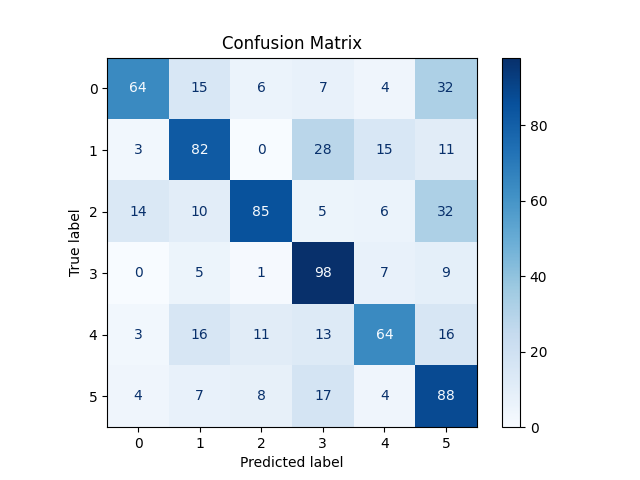
\includegraphics[width=1.0\linewidth]{../resources/crnn_confusion.png}
      \caption{Confusion matrix of CRNN model. The categories are the same 
      as \autoref{fig:baseline_confusion}.} 
      \label{fig:crnn_confusion}
    \end{minipage}
\end{figure}

\end{document}